\section{Androidin mukana tulevista työkaluista}

Pitäiskö tässä luvussa olla jotain ylipäänsä testaamisen perusteita, vai riittääkö että johdannossa sivutaan aihetta?

\subsection{Android SDK:n mukana tulevia testityökaluja}

\begin{figure}[htb]
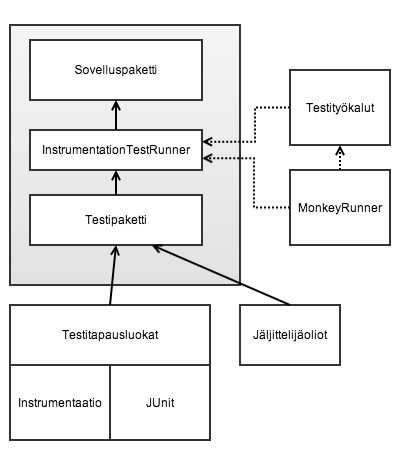
\includegraphics[width=100mm]{test_framework.png}
\caption{placeholder omalle kuvalle} \label{test_framework}
\end{figure}

Androidin SDK:n (suomennos!) mukana tulee monia testaustyökaluja. Testejä voi ajaa joko emulaattorilla tai suoraan puhelimessa.

Androidin testisarjat(suite?) perustuvat JUnit-työkaluun. Puhdasta JUnitia voi käyttää sellaisen koodin testaamiseen, joka ei kutsu Androidin rajapintaa tai sitten voi käyttää Androidin JUnit-laajennusta Android-komponenttien testaukseen. Laajennus tarjoaa komponenttikohtaiset test case (suomennos?) luokat. Nämä luokat tarjoavat apumetodeita mock-olioiden(suomennos?) luomiseen ja komponentin elinkaaren hallintaan. Androidin JUnit-toteutus mahdollistaa JUnitin versio 3:n mukaisen testityylin, ei uudempaa versio 4:n mukaista.

Kuvassa \ref{test_framework} on esitetty Androidin testien ajoympäristö. Testattavaa sovellusta testataan ajamalla testipaketissa olevat testitapaukset MonkeyRunnerilla (ks. luku \ref{monkeyrunner}). Testipaketti sisältää testitapausten lisäksi Androidin instrumentaatiota, eli apuvälineitä sovelluksen elinkaaren hallintaan ja koukkuja, joilla järjestelmän lähettämiä callback-metodikutsuja pääsee muokkaamaan, sekä mahdollisesti mock-olioita korvaamaan järjestelmän oikeita luokkia testin ajaksi mock-toteutuksella. \cite{android}

\subsection{Komponenttikohtaiset testiluokat}

Android tarjoaa aktiviteeteille, palveluille ja sisällöntarjoajille jokaiselle oman testiyläluokkansa, joka mahdollistaa komponenttikohtaisten testien helpomman toteutuksen.

Aktiviteettien testauksessa Androidin JUnit-laajennus on tärkeä, koska aktiviteeteilla on monimutkainen elinkaari, joka perustuu paljolti callback-metodeihin (suomennos), joiden suora kutsuminen ei ole mahdollista. Aktiviteettien testauksen pääyläluokka on InstrumentationTestCase. Sen avulla on mahdollista käynnistää, pysäyttää ja tuhota testattavana oleva aktiviteetti halutuissa kohdissa. Lisäksi sen avulla voi mockata järjestelmäolioita, kuten Contexteja ja Applicationseja. Tämä mahdollistaa testin eristämisen muusta järjestelmästä ja Intentien luomisen testiä varten. Lisäksi yliluokassa on metodit käyttäjäinteraktion, kuten kosketus- ja näppäimistötapahtumien lähettämiseen suoraan testattavalle luokalle.

Aktiviteettien testaamiseen on kaksi olennaista välitöntä yliluokkaa, ActivityUnitTestCase ja ActivityInstrumentationTestCase2. ActivityUnitTestCase on tarkoitettu luokan yksikkötestaamiseen siten, että se on eristetty Android-kirjastoista. Näitä testejä voi ajaa suoraan IDEstä ja tarvittaessa Android-kirjaston mockaamiseen on käytössä MockApplication-olio. ActivityInstrumentationTestCase2 taas on tarkoitettu toiminnalliseen testaukseen tai useamman aktiviteetin testaamiseen. Ne ajetaan normaalissa suoritusympäristössä emulaattorilla tai Android-laitteessa. Aikeiden mockaus on mahdollista, mutta testin eristäminen muusta tuotantojärjestelmästä ei ole mahdollista.

Palveluiden testaaminen on paljon yksinkertaisempaa kuin aktiviteettien. Ne toimivat eristyksessä muusta järjestelmästä, joten testattaessakaan ei tarvita Androidin instrumentaatiota. Android tarjoaa ServiceTestCase-yliluokan palveluiden testaamiseen. Se tarjoaa mock-oliot Application- ja Context-luokille, joten palvelun saa testattua eristettynä muusta järjestelmästä. Testiluokka käynnistää testattavan palvelun vasta kutsuttaessa sen startService() tai bindService()-metodia, jolloin mock-oliot voi alustaa ennen palvelun käynnistymistä. Mock-olioiden käyttö palveluiden testaamisessa paljastaa myös mahdolliset huomaamatta jääneet riippuvuudet muuhun järjestelmään, koska mock-oliot heittävät poikkeuksen, mikäli niihin tulee metodikutsu, johon ei ole varauduttu.

Sisällöntarjoajien testaaminen on erityisen tärkeää, jos sovellus tarjoaa sisällöntarjoajiaan muiden sovellusten käyttöön. Tällöin on myös olennaista testata niitä käyttäen samaa julkista rajapintaa, jota muut sovellukset joutuvat käyttämään kommunikoidessaan sisällöntarjoajien kanssa. Sisällöntarjoajien testauksen yliluokka on ProviderTestCase2, joka tarjoaa käyttöön mock-oliot ContentResolveriosta ja Contextista, jolloin sisällöntarjoajia voi testaja eristyksissä muusta sovelluksesta. Yliluokka tarjoaa myös metodit sovelluksen oikeuksien testaamisen. Contextin mock-olio mahdollistaa tiedosto- ja tietokantaoperaatiot, mutta muut Androidin kirjastokutsut on toteutettu stubeina. Lisäksi tiedon kirjoitusosoite on uniikki testissä, joten testien ajaminen ei yliaja varsinaista sovelluksen tallentamaa tietoa. Sisällöntarjoajatestit ajetaan emulaattorissa tai Android-laitteella. \cite{android}

\subsection{MonkeyRunner}
\label{monkeyrunner}

MonkeyRunner tarjoaa rajapinnan, jolla android-sovellusta voi ohjata laitteessa tai emulaattorissa. Se on lähinnä tarkoitettu toiminnallisten testien (functional tests, onko oikea suomennos?) sekä yksikkötestien ajamiseen, mutta soveltuu myös muihin tarkoituksiin. Sen avulla voi esimerkiksi asentaa sovelluksia, ajaa testisarjoja ja sovelluksia ja lähettää niihin syötteitä. Lisäksi monkeyrunnerilla voi ottaa eri kohdista kuvakaappauksia ja verrata niitä referenssikuviin. Tällä tavalla voidaan tehdä esimerkiksi regressiotestausta.

MonkeyRunnerilla voidaan testata yhtä aikaa esimerkiksi monia eri emulaattoreita tai useita laitteita, jolloin voidaan tehdä fragmentaatiotestausta. MonkeyRunner on myös laajennettavissa, jolloin sitä voi käyttää muihinkin tarkoituksiin. MonkeyRunneria ohjataan pythonilla ja se on toteutettu jythonilla, joka on Javan virtuaalikoneessa pyörivä python-toteutus.\cite{android}

\subsection{Uiautomator ja uiautomatorviewer}

Monkeyrunneria paremmat assert-mahdollisuudet ja mahdollisuuden toiminallisten mustalaatikko-testien kirjoittamiseen Javalla tarjoaa uiautomator. Siinä on kaksi komponenttia uiautomatorviewer ja uiautomator. Uiautomatorviewer on graafinen työkalu, jolla voi analysoida ja skannata Android-sovelluksen käyttöliittymää ja uiautomator työkalu, joka tarjoaa rajapinnan ja moottorin toiminnallisten mustalaatikkotestien ajamiseen.

\begin{figure}[htb]
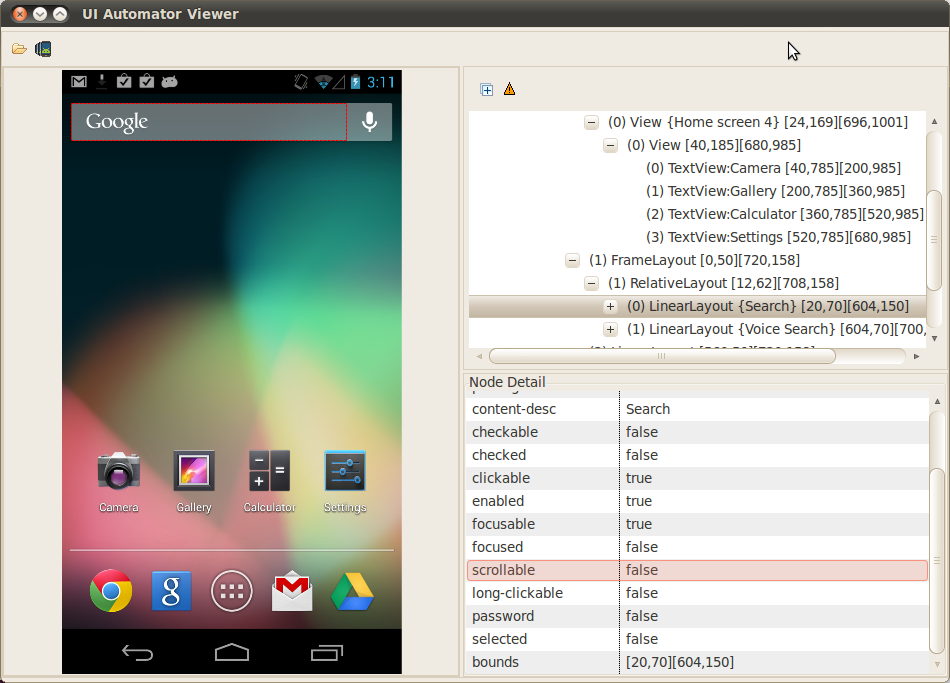
\includegraphics[width=150mm]{uiautomatorviewer.png}
\caption{placeholder omalle kuvalle} \label{uiautomatorviewer}
\end{figure}

Uiautomatorviewer (kuvassa \ref{uiautomatorviewer}) blah

\cite{android}

\subsection{Monkey}

Monkey on Androidin mukana tuleva työkalu, jota voi ajaa emulaattorissa tai Android-laitteessa ja joka tuottaa pseudosatunnaisia syötteitä ohjelmalle, kuten painalluksia, eleitä sekä järjestelmätason viestejä. Monkeytä voi käyttää esimerkiksi sovelluksen stressitestaukseen tai fuzz-testaukseen.

Monkeylle voi antaa jonkin verran sen toimintaa ohjaavia parametreja. Ensinnäkin testisyötteiden määrää ja tiheyttä voi rajoittaa. Toiseksi erityyppisten syötteiden osuutta voi säätää. Kolmanneksi testauksen voi rajoittaa tiettyyn pakettiin sovelluksessa. Tällöin Monkey pysäyttää testauksen, jos se on ajautuu muihin kuin haluttuun osaan sovelluksesta. Neljänneksi Monkeyn tulosteiden määrää ja tarkkuutta voi säätää.

Monkey pystäyttää testin, jos ohjelmasta lentää käsittelemätön poikkeus tai jos järjestelmä lähettää sovellus ei vastaa -virheviestin. Näissä tapauksissa Monkey antaa raportin virheestä ja miten se syntyi. Monkey voi myös haluttaessa tehdä profilointiraportin testistä.\cite{android}

\subsection{Androidin fragmentaatio}

Google tarjoaa android-laitteiden fragmentaation seurantaan palvelua, jossa kerrotaan kahden viikon jaksolla Androidin sovelluskaupassa käyneiden laitteiden jakauma androidin version, näytön koon ja resoluution sekä OpenGL:n version mukaan.\cite{android_versions} Jakauma ei välttämättä vastaa käytössä olevien Android-laitteiden jakaumaa, mutta toisaalta sovelluskehittäjän kannalta ne käyttäjät, jotka käyttävät sovelluskauppaa, lienevät olennaisimpia.

\begin{table}[h]
\centering
\begin{tabular}{ l l l l }
  Versio & Koodinimi & API & Osuus \\
  1.5 & Cupcake & 3 & 0.1\% \\
  1.6 & Donut & 4 & 0.4\% \\
  2.1 & Eclair & 7 & 3.4\% \\
  2.2 & Froyo & 8 & 12.9\% \\
  2.3 - 2.3.2 & Gingerbread & 9 & 0.3\% \\
  2.3.3 - 2.3.7 & Gingerbread & 10 & 55.5\% \\
  3.1 & Honeycomb & 12 & 0.4\% \\
  3.2 & Honeycomb & 13 & 1.5\% \\
  4.0.3 - 4.0.4 & Ice Cream Sandwich & 15 & 23.7\% \\
  4.1 & Jelly Bean & 16 & 1.8\% \\
\end{tabular}
\caption{Androidin versioiden osuus 1.10.2012 päättyneellä 2-viikkoisjaksolla}
\label{tab:android_versions}
\end{table}

Taulukko \ref{tab:android_versions} kuvaa androidin käyttöjärjestelmäversioiden jakaumaa. Miksi olennainen? Androidin 4-versio julkaistiin lokakuussa 2011, mutta vuotta myöhemmin vain noin neljäsosa laitteista käyttää 4. versiota. Jos sovelluskehittäjä haluaa tukea esimerkiksi 90\% markkinoilla olevista laitteista, on tuki ulotettava 2.2-versioon, joka julkaistiin toukokuussa 2010. \cite{android_version_history}

\begin{table}[h]
\centering
\begin{tabular}{ l l l l l }
   & ldpi (~120dpi) & mdpi (~160dpi) & hdpi (~240dpi) & xhdpi (~320dpi) \\
  small & 1.7\% &  & 1.0\% &  \\
  normal & 0.4\% & 11\% & 50.1\% & 25.1\% \\
  large & 0.1\% & 2.4\% &  & 3.6\% \\
  xlarge &  & 4.6\% &  &  \\
\end{tabular}
\caption{Android-laitteiden näyttökokojen ja pikselitiheyden osuudet 1.10.2012 päättyneellä 7 päivän jaksolla.}
\label{tab:screen_sizes}
\end{table}

Android-laitteet poikkeavat toisistaan sekä näytön fyysisen koon, että pikselitiheyden puolesta. Taulukossa \ref{tab:screen_sizes} on kuvattuna erilaisten näyttötyyppien jakaumaa. Näytön koon arvioinnissa android käyttää tiheysnormalisoituja pikseleitä (Density-independent pixel, dp), jotka lasketaan kaavalla px = dp * (dpi / 160), missä px on pikseli ja dpi on pikseleiden määrä tuumalla. Siten esimerkiksi 240 dpi:n näytöllä, yksi dp vastaa puoltatoista fyysistä pikseliä. Sovellusten ulkoasu tulisi aina suunnitella käyttäen dp:tä yksikkönä, jolloin skaalaus eri kokoisille ja pikselitiheyksisille näytöille onnistuu parhaiten. Taulukossa \ref{tab:screen_sizes} näyttökoot on lajiteltu niin, että xlarge näyttöjen resoluutio on vähintään 960dp x 720dp, large: 640dp x 480dp, normal: 470dp x 320dp ja small vähintään 426dp x 320dp.

\begin{table}[h]
\centering
\begin{tabular}{ l l }
  OpenGL ES versio & jakauma \\
  1.1 & 9.2\% \\
  2.0 \& 1.1 & 90.8\% \\
\end{tabular}
\caption{OpenGL versiot}
\label{tab:opengl_versions}
\end{table}

Taulukossa \ref{tab:opengl_versions} on kuvattu OpenGL ES -versioiden jakauma Android-laitteissa.\cite{android_versions}

Oheisten muuttujien lisäksi Android-laitteet poikkeavat toisistaan myös monilla muilla tavoin. Suoritintehoa laitteissa on hyvin eri määrissä käytössä ja näytönohjainten tehotkin vaihtelevat. Lisäksi erilaisia lisälaitteita, kuten gps, kiihtyvyysantureita, kompasseja yms. saattaa olla laitteissa, tai olla olematta.

\subsection{Mitä keinoja android sdk tarjoaa fragmentaation hallintaan}

Jos sovellus tarvitsee välttämättä laitteelta tiettyjä ominaisuuksia, on mahdollista suodattaa sovellus pois Androidin sovelluskaupan hauista, jos sitä haetaan laitteella, joka ei tue sovelluksen vaatimia ominaisuuksia. Tärkeimmät suotimet ovat androidin API:n minimiversio, tiettyjen lisälaitteiden olemassaolo ja näytön koko.

<uses-sdk>-direktiivillä (directive suomennos?) määritellään Androidin APIn minimiversio. Jos laitteessa on käytössä pienempi API-versio kuin direktiivillä annettu, sovellusta ei näytetä hakutuloksissa. <support screens>-direktiivi määrittelee, millä näytön koolla sovellus toimii. Tavallisesti määrittelemällä jokin tuettu koko, sovelluskauppa olettaa, että laite tukee sen lisäksi myös isompia näyttökokoja, muttei pienempiä. On myös mahdollista määritellä erikseen kaikki tuetut näyttökoot.

<uses-feature>-direktiivillä voidaan määritellä mitä ominaisuuksia sovellus vaatii. Näitä on sekä laitteistotasolla, kuten kamera, kiihtyvyysanturi tai kompassi, että ohjelmistotasolla, kuten vaikka liikkuvat taustakuvat, joiden pyörittämiseen kaikissa Android-laitteissa ei riitä resursseja. <uses-feature>-direktiiviä käytetään, kun sovellus ei lainkaan toimi ilman kyseistä ominaisuutta. Jos sovellus on käyttökelpoinen myös ilman ominaisuutta, voi tämän hallintaan käyttää muita keinoja (ja ne oli..?)  \cite{android_compatibility}